\begin{figure}[tb]
\center{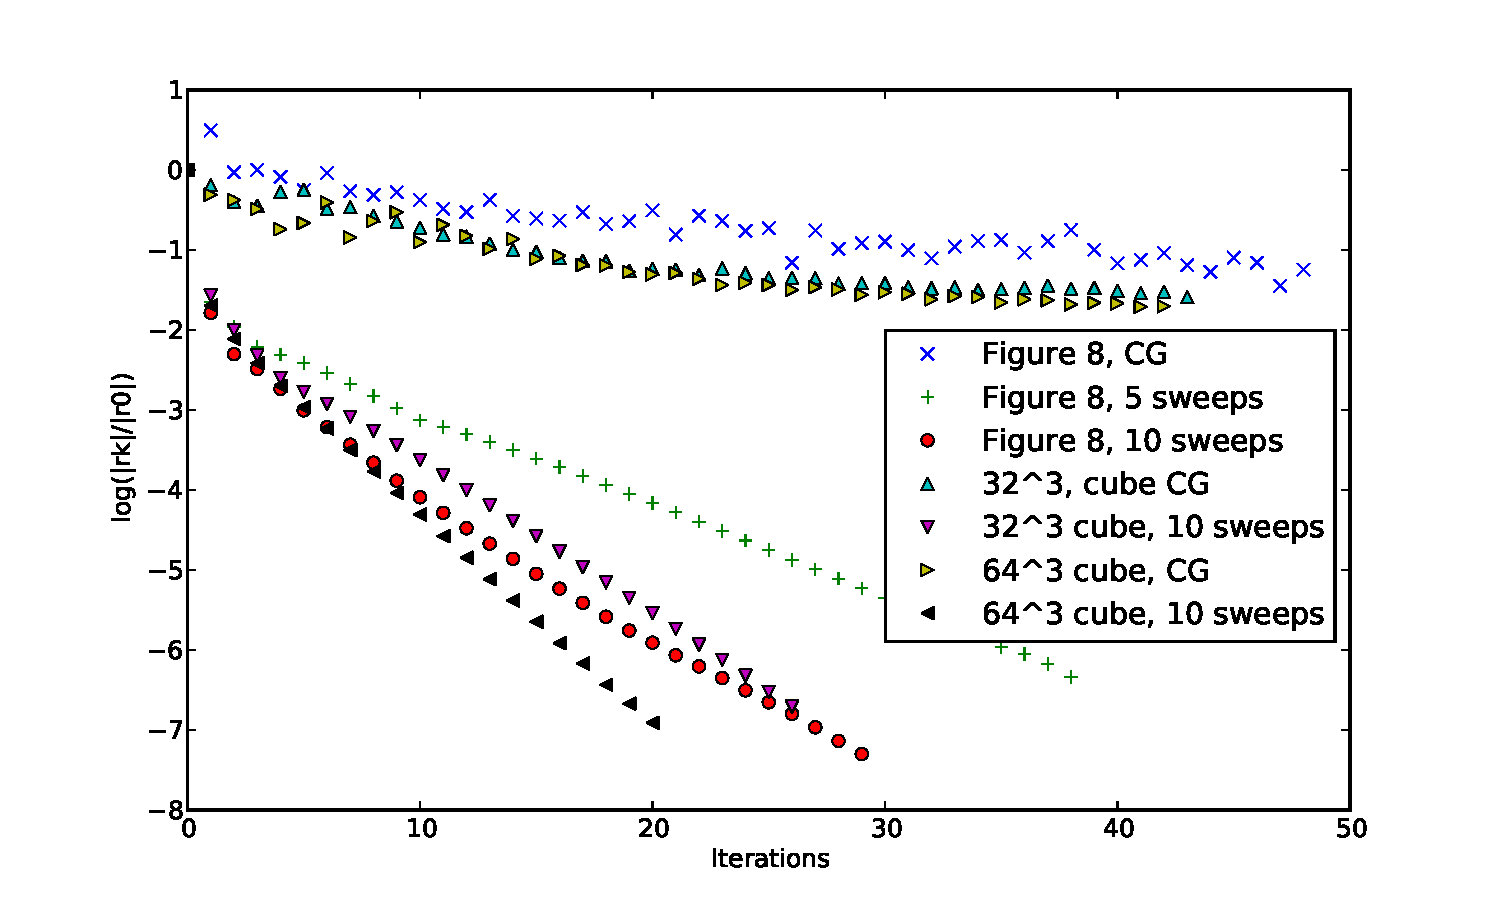
\includegraphics[width=.8\linewidth]{elasticity/figures/convergence_plot.pdf}}
\caption[Residual reduction $|r_k|_{\infty}/|r_0|_{\infty}$ per
  V-cycle or CG iteration for a number of examples.]{Residual reduction $|r_k|_{\infty}/|r_0|_{\infty}$ per
  V-cycle or CG iteration for a number of examples. In practice 1-3 v-cycles were necessary for each  Newton-Raphson update}
\label{fig:cube_convergence}
\end{figure}


We tested our full system on a number of production-quality models, focusing on regions where artists typically struggle to achieve realistic, collision-free results using traditional rigging methods.  

\subsection{Setup}
\begin{figure}[tb]
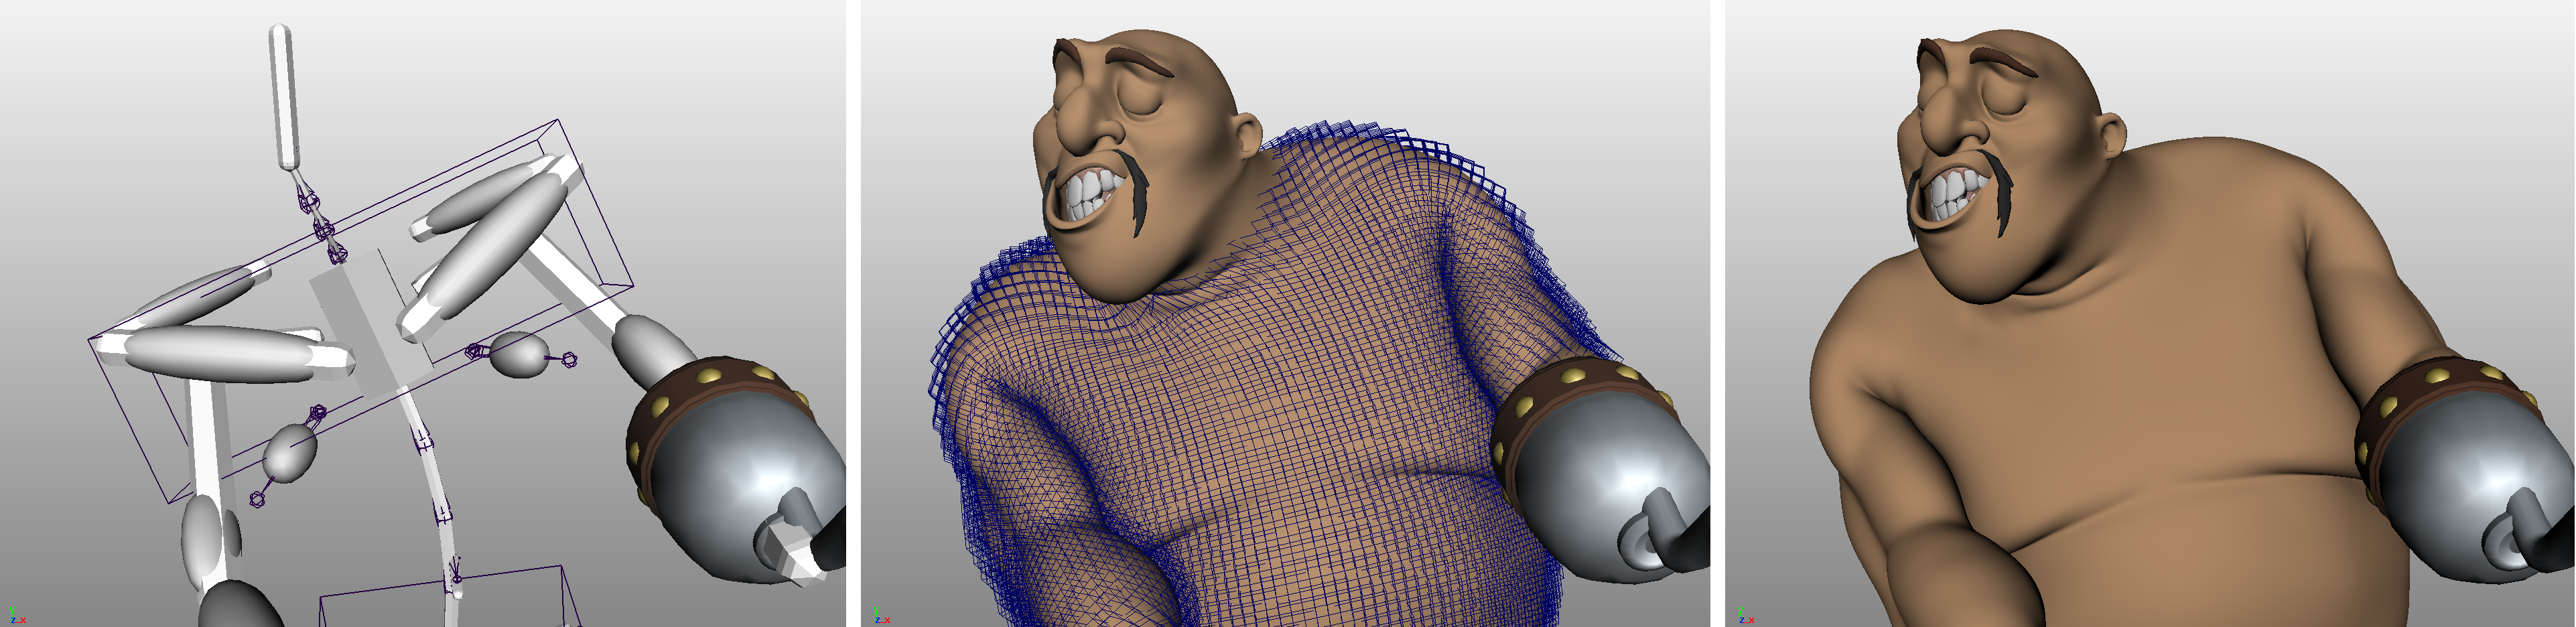
\includegraphics[width=\linewidth]{elasticity/figures/teaser3}
 \caption[The setup procedure for our method.]{Our method takes a geometric internal skeleton (left) and a source
   surface mesh (not pictured) as input. Based on a hexahedral lattice (center)
   it then simulates a deformed surface (right) obeying self-collision and volumetric
   elasticity. The example shown here has 106,567 cells and simulates at 5.5
   seconds per frame. Images \copyright Disney. All rights reserved.}\label{fig:teaser}
\end{figure}
Our simulation is driven by rigid bones attached to the character's existing skeleton.  Simple geometric shapes such as cylinders or ellipsoids are sufficient to define the volumetric extent of these bones, and we found that using soft constraints with narrow bones gave the elasticity model freedom to produce appealing flesh-like shapes. More carefully modeled bones can be used as internal collision objects over which the material can slide, providing detail in regions such as the elbow or around the collarbone. Finally, our self collision handling not only prevents interpenetration, it also works with our elastic simulation to create realistic squishing and bulging behavior.  

In addition to these basic features, in our examples we allow our deformer to be applied to sub-regions of the character mesh. Soft constraints ``stitch'' the simulation region to the underlying mesh in blend regions, allowing for a seamless transition.  

For highly stylized characters, detailed underlying structures such as muscles and tendons are often unclear or at least time consuming to create. By supporting spatially varying material parameters, we are able to easily approximate many of these coarse grain features.  Our interface allows users to paint material parameters onto the surface mesh; the parameters are then extrapolated to the volume by solving a Laplace equation.  Whereas we often attain acceptable results with constant material parameters, we can better sculpt shapes by varying the stiffness and Poisson's ratio of the material.

\subsection{Examples}
\begin{figure*}[tb]
\center{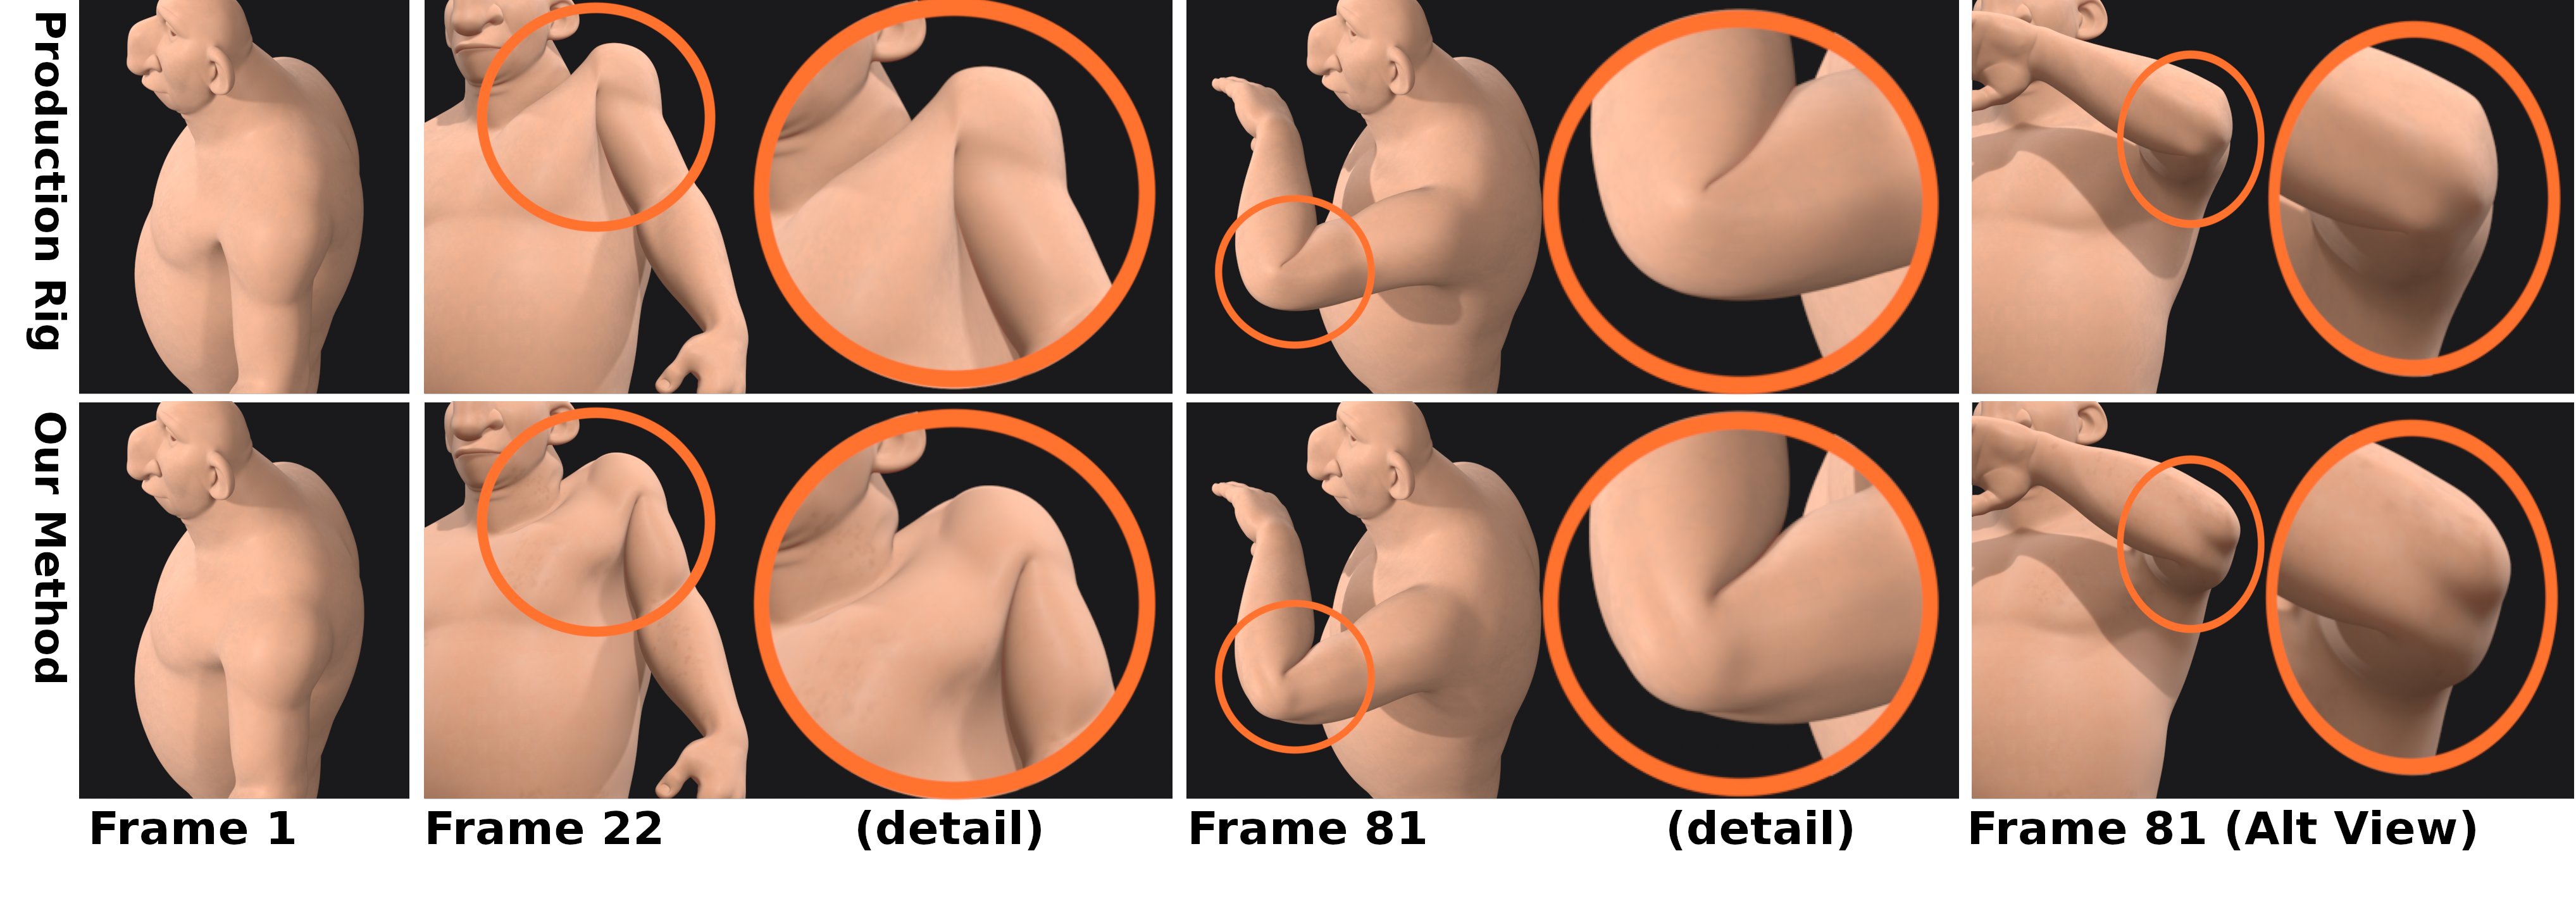
\includegraphics[width=\linewidth]{elasticity/figures/thugfigure}}
\caption[A comparison with linear blend skinning on a character arm
  and shoulder.]{A common problem with many existing techniques (and linear blend
  skinning in particular) is that it can be very difficult to maintain the
  illusion of an underlying bone-structure. As an example the top row here shows
  how the integrity of the region around the clavicle is lost as the character
  shrugs. In the bottom row, however, everything behaves as a connected
  entity. On the outside of the elbow we also get a nice protrusion of the ulna
  with our method as opposed to the more rubber-like behavior of the linear
  blend skin. The simulation here is based on 30,904 non-empty cells. Images \copyright Disney. All rights reserved.}
\label{fig:thug}
\end{figure*}
In all examples, we found that 1-2 V-cycles with 5 relaxation sweeps
per grid transfer were sufficient for the linear solver.  The number
of Newton iterations required depended on our initial guess; when
using the previous frame of an animation, we typically required
between 1 and 10 iterations for full convergence.  All reported CPU
times were computed on an 8-core Intel Xeon X5550 workstation.  GPU
tests were performed on an NVIDIA Quadro 6000. For interactive use it
should be noted that faster feedback can be provided by progressively
updating the display after each Newton iteration.

In Figure~\ref{fig:cube_convergence}, we compare convergence rates per
V-cycle or conjugate gradients iteration for a number of examples.  We
suspect that initial ``bump'' in residual reduction per V-cycle can be
explained by the efficiency of our Jacobi smoother.  We note that a
constant convergence rate emerges for all multigrid examples, in
contrast with CG.

In our first example, we applied our deformer to the arm, shoulder and neck region of a character (see Fig. \ref{fig:thug}). Each Newton iteration averaged 0.492s on the CPU and 0.345s on the GPU.  Our average frame times were 3.22s and 2.38s on the CPU and GPU respectively.

In Figure \ref{fig:hand}, we demonstrate our method on a character hand.  On the CPU, we averaged 1.40s per Newton iteration for an average of 12.6s per frame.  On the GPU, each Newton iteration averaged  0.612s for an average of 5.74s per frame.

Finally, in Figure~\ref{fig:teaser} we apply our deformer to the torso and arms of a large character with 106,567 elements. On the CPU, each Newton iteration was approximately 0.876s for a total of 5.48s per frame.  Our GPU implementation averaged 0.762s per Newton iteration and 5.14s per frame.
